\documentclass{./llncs2e/llncs}
\usepackage{graphicx}
\usepackage{float}
\usepackage{mathtools}
\usepackage[utf8]{inputenc}
\usepackage[nolist,nohyperlinks]{acronym}
% Maintain images and tables within their respective sections
\usepackage[section]{placeins}
\usepackage{array}

\usepackage[hyphens]{url}
\usepackage[hidelinks]{hyperref}
\hypersetup{breaklinks=true}

%\usepackage{amssymb}% http://ctan.org/pkg/amssymb
\usepackage{pifont}% http://ctan.org/pkg/pifont
\newcommand{\cmark}{\ding{51}}%
\newcommand{\xmark}{\ding{55}}%

%\usepackage{refcheck}
%
% Change the margins
%
% \usepackage[margin=2.9cm]{geometry}

\begin{document}
\title{TrubiZone}

\subtitle{Securing Critical Mobile Applications for Android Using ARM TrustZone}
\author{Tiago Brito\\
Supervisor: Prof. Nuno Santos}

\institute{Instituto Superior Técnico,\\
Av. Rovisco Pais, 1049-001 Lisboa - PORTUGAL\\
\textbf{tiago.de.olveira.brito@tecnico.ulisboa.pt}}

\maketitle

% make a proper TOC despite llncs
%\setcounter{tocdepth}{2}
\setcounter{secnumdepth}{3}
\setcounter{tocdepth}{3}
\makeatletter
\renewcommand*\l@author[2]{}
\renewcommand*\l@title[2]{}
\makeatletter

%\cleardoublepage
%!TEX root = ../report.tex

% 
% Abstract 
% 

\begin{abstract}

Mobile devices are growing and being adopted everywhere. Increasingly, such devices execute critical applications which require very sensitive data to be displayed on the devices' screen, for example medical and financial records, which are commonly processed by mHealth and e-money apps, respectively. But, in order to display sensitive information to the user, applications currently depend not only on their own code but also in the code of all underlying layers, which include a full-blown operating system. Given that all these software layers result in a very large and complex computing base, it is difficult to ensure that the sensitive application records displayed on screen have not been intercepted and leaked by a malicious agent that has managed to compromise the operating system. The goal of this thesis is to design and implement a solution that enables applications to securely output sensitive data without relying on a native rich OS, but rather depend on a very small amount of trusted software code isolated from the rich OS using ARM's secure hardware technology, TrustZone. This report describes the state of the art and introduces a preliminary architecture of our solution: a software system named ViewZone. To motivate and validate the concept of this solution, a critical mobile health application will be implemented.

\end{abstract}
%%!TEX root = ../report.tex

% 
% Keywords 
% 

\begin{keywords}

TrubiZone, Security, Privacy, e-Health, Mobile Devices, Android, TrustZone

\end{keywords}

%\cleardoublepage
%\tableofcontents
%\cleardoublepage
\pagestyle{plain}
\pagenumbering{arabic}
%!TEX root = ../report.tex

% 
% Introduction
% 

\section{Introduction (2/3pgs)}

General description of the problem and its context, current solutions, and road map of the project.

According to Comscore's 2015 "Digital Future in Focus" whitepaper, with key statistics for the U.S. market, mobile devices, such as smart-phones and tablets, dominate digital media time over the PC, with the trend being to continue raising. This shows in the near future we maybe living in a world where mobile devices are the predominant device.
%\cleardoublepage
%%!TEX root = ../report.tex

% 
% Objectives
% 

\section{Objectives (1pg)}

Clearly explain the project objectives.

%\cleardoublepage
%!TEX root = ../report.tex

% 
% Related work
% 
% (~17pgs)
\section{Related Work}
\label{sec:relatedWork}

This section describes the related work and is organized in three main parts: mobile health security, general-purpose mobile security mechanisms and TrustZone-based systems.
%FIRST
In order to understand the necessity for secure input and display in critical mobile applications, we must introduce a class of apps which benefit from such security improvements. As a representative example of such as class of applications is the mobile health sector. For this reason, the first part focuses presenting the main studies in mobile health security. In particular, it describes the attack surfaces of mHealth apps, the most common threats and their seriousness.
%SECOND
In the second part of this section, we overview the state of the art of general-purpose mobile security mechanisms used to implement most secure-sensitive applications, such as those described in the first part. We also explain why such mechanisms fall short in supporting secure output to these apps.%with a particular focus on the Android Operating System.
%THIRD
Finally, the third part describes a specific class of security systems which, similarly to \emph{ViewZone}, leverage TrustZone to implement a variety of security solutions for mobile platforms.

\subsection{Studies in Mobile Health Security}
\label{sec:mhealth}

Medical data is highly profitable for malicious agents who use it for medical identity theft, as it can be more valuable than credit card information. Generally, vulnerabilities which lead to sensitive data leakage originate from negligent development of healthcare systems. For this reason, regulatory laws such as the \ac{HIPAA} have been established. These laws comprise the standard for electronic healthcare transactions and must be followed by all developers when managing sensitive health data.

In the mobile context, data is even more exposed and vulnerable due to the inherent portability of these devices, the sharing of information to third-party advertisers by device manufacturers or mobile app developers, unregulated management of sensitive medical information, specially because regulatory laws such as \ac{HIPAA} do not account for the mobile sector, and because of security flaws on consumer device software, which may lead to a malware compromised system. This is why there is a need for a novelty security system capable of allowing applications to securely display and manage sensitive data.

The following subsections describe work done in assessing the current security state of the art of commercial mobile health applications as to better understand the need for a secure content display capability. The first subsection describes a threat taxonomy for mHealth applications by Kotz et al.~\cite{kotz2011threat}. The second and third subsections describe work done by He et al.~\cite{he2014security} through the analysis of three studies which answer the following questions: what are the potential attack surfaces, how widespread and how serious are the security threats to mobile health applications.

\subsubsection{Threat Taxonomy for Mobile Health Applications}

Kotz et al.~\cite{kotz2011threat} defines a threat taxonomy for mHealth and categorizes threats in three main categories: \emph{identity threats}, \emph{access threats} and \emph{disclosure threats}.

\emph{Identity threats} are described as a mis-use of patient identities and include scenarios where a patient may lose (or share) their identity credentials, allowing malicious agents to access their respective \ac{PHR}. \emph{Insiders} (authorized \ac{PHR} users, staff of the \ac{PHR} organization or staff of other mHealth support systems) may also use patient identities for medical fraud or for medical identity theft, and \emph{outsiders} may be able to observe patient identity or location from communications.
%tempo verbal no their? nao entendi

\emph{Access threats} are described as unauthorized access to \ac{PHR} and include scenarios where the patient, which controls the data, may allow broader-than-intended access or disclosure of information, \emph{insiders} who may snoop or modify patient data with malicious intent, and even \emph{outsiders} which, by breaking into patient records, may leak or modify this data.
% QUEREMOS RESOLVER ESTES

\emph{Disclosure threats} include scenarios where an adversary captures network packets in order to obtain sensitive health data. This problem can be mitigated by using strong encryption methods, but even if the network traffic is encrypted it is possible to analyse the traffic to determine its characteristics~\cite{wright2006inferring}. The adversary may also use physical-layer, or link-layer fingerprinting, methods to identify the device type and, because the wireless medium is open, an active adversary may inject frames or may selectively interfere (cause collisions) with wireless frames.

Avancha et al.~\cite{avancha2012privacy} developed a privacy framework for mHealth and discussed the technologies that could support privacy-sensitive mobile health systems. A developer should use the list of privacy properties provided by this article as a check-list to be considered in any design. But even these security properties are not sufficient to withstand an attack leveraged by a compromised operating system, which is an attack not explicitly described above. For this reason, there is a need for a security solution capable of withstanding such attacks whilst protecting sensitive information.
 
\subsubsection{Potential Attack Surface of Commercial Mobile Health Applications}

He et al.~\cite{he2014security} analyse several mHealth applications available in Android's app store to contribute to the understanding of security and privacy risk on the Android platform. In the first of three studies described, 160 apps were analysed to find evidence of security threats. From surveying previous literature, seven attack surfaces, shown in Table~\ref{tab:attacksurfaces}, are determined to be in need of protection.

\begin{table}[t]
	\caption {Description of attack surface (taken from He et al. \cite{he2014security})}
	\label{tab:attacksurfaces}
	\begin{tabular}{|>{\raggedright}p{2cm}|>{\raggedright\arraybackslash}p{10cm}|}
		\hline
		\textbf{Attack Surface}      & \textbf{Description}                                                                                                                    \\ \hline
		Internet            & Sensitive information is sent over the internet with unsecure protocols (e.g. HTTP), misconfigured HTTPS, etc.                 \\ \hline
		Third Party         & Sensitive information is stored in third party servers                                                                         \\ \hline
		Bluetooth           & Sensitive information collected by Bluetooth-enabled health devices can be sniffed or injected                                 \\ \hline
		Logging             & Sensitive information is put into system logs where it is not secured                                                          \\ \hline
		SD Card Storage     & Sensitive information is stored as unencrypted files on SD card, publicly accessible by any other app                          \\ \hline
		Exported Components &  Android app components, intended to be private, are set as exported, making them accessible by other apps                     \\ \hline
		Side Channel        & Sensitive information can be inferred by a malicious app with side channels, e.g. network package size, sequence, timing, etc. \\ \hline
	\end{tabular}
\end{table}

Table~\ref{tab:attacksurfaces} is an overview of the problems disclosed by the apps studied, where applications send unencrypted information or use misconfigured internet protocols, store data in third-party server, where data is not assured to be secure, inadvertently log sensitive data to the system or export private app components making them accessible to other applications. Table~\ref{tab:attacksurfaces} is missing an important attack surface, which is the operating system. Although usually well protected and in constant update to mitigate vulnerabilities found in previous versions, operating systems have an extensive and complex code base, and there are no security guarantees that the system will never be compromised by malware, which can then control system resources and the overlying applications. Resources, such as the framebuffers or touchscreen device, might be explored by a malicious agent in order to disclose data, such as sensitive medical information.

The authors also document that most apps targeted for patients (60\%) are in the Life Management category, which comprises apps such as nutrition apps and workout apps, followed by apps that manage and synchronize user health information (\ac{PHR} Management), which occupy nearly half (46.88\%) of these applications. These numbers are a good indicator of the data handled by most commercial mHealth apps available as well as which health apps are more used in the mobile health sector. These numbers also motivate the choice made to build a personal health record management app, implemented using \emph{ViewZone}, in order to demonstrate the security solution features and properties, namely secure display, input and storage of sensitive data.

\subsubsection{Severity of Attacks to Mobile Health Applications}
In the second study by He et al.~\cite{he2014security}, 27 of the top 1080 free apps from the Medical and Health \& Fitness categories on Google Play were analysed in order to assess the most common observed vulnerabilities. To achieve this, the authors analyse what data is achievable by an agent acting maliciously. From this analysis, three attack surfaces are identified as the most important ones: \emph{Internet}, \emph{Third Party Services} and \emph{Logging} (see Table~\ref{tab:attacksurfaces}).

Only 7 of these 27 apps use the Internet to effectively send medical information over to remote servers. Some of these apps sent unencrypted content over the Internet, which generally include emails, usernames and passwords. This study also concludes that most of these apps are hosted, and store the recorded data, on third party servers. This is an economical and scalable solution for mobile applications, but storing sensitive health records on third party servers can have serious implications, mostly due to app users not being aware that their data is being stored on third party servers and because these users are incapable of telling whether this data is encrypted in such a way that hosting companies do not have access to it.

In the third study by He et al.~\cite{he2014security}, another 22 apps, which send information over the Internet, are randomly selected from the same top 1080 apps and audited to understand what information is effectively being sent over the Internet, thus inferring the seriousness of the threats. The conclusion is that, when used as intended, these apps gather, store and transmit a variety of sensitive user data, which includes at least personal profiles, health sensor data, lifestyle data, medical browsing history and third-party app data (e.g. Facebook account information).

The consequences of data breaches, information disclosure or tempering with sensitive health data depend on the type, sensitivity and volume of data breached, but it is clear that profiling, medical identity theft and healthcare decision-making errors are all possible. This is why the authors suggest the use of encryption for communication and storage, and encourage developers to create a set of standard security and privacy guidelines that offer a baseline for protection. However, these measures are not sufficient to protect sensitive data against more complex attacks, such as those which involve a malware compromised operating system. In such a system, where the malicious entity controls system resources, encryption techniques and good developing guidelines for critical applications might not be enough as the system can bypass these mechanisms and disclose data when it is in its raw displayable for, i.e., unencrypted.\\

Security measures and regulatory laws are implemented for custom healthcare information systems in order to mitigate attacks which may disclose sensitive medical data. However, in the mobile sector, these security measures may not be possible or practical to implement, and regulatory laws, such as \ac{HIPAA}, do not account for the mobile market. For this reason, the research community analysed and categorized mHealth sector threats, developed a privacy framework and studied commercially available applications in order to achieve a standardized set of rules to mitigate negligent development. But these studies consider the whole operating system as the trusted computing base for mobile health apps, and, because this \ac{TCB} e so complex and unreliable, malware may take control of system resources and consequently leak sensitive data. Ultimately, what the mHealth market needs is a security solution which provides the secure primitives, which both developers and users desire, such as secure display, input and storage, without having to rely on a full-featured operating system, inherently with a large \ac{TCB}.

\subsection{General-Purpose Mobile Security Mechanisms}

This section describes the security mechanisms available for the Android platform, either native or as security extensions, and how these mechanisms can be used to solve some of the problems covered in the previous section. Since many security mechanisms have been proposed, we divide them into groups to reflect the different ways in which sensitive information is protected: \emph{(a)} access control mechanisms enforce security policies that prevent access to sensitive resources by a given application, \emph{(b)} application communication monitoring ensures that sensitive data that was read by a given application can be securely exchanged with co-located applications, \emph{(c)} privacy enhancement systems aim to prevent privacy breaches by applications that have read from sensitive resources and need to share that data with Internet services, and \emph{(d)} trusted execution systems provide restricted environments in which security-sensitive data can be processed while trusting in a smaller amount of code than in the typical system operation. Figure~\ref{fig:relwork} maps these four groups to a representation of a possible mobile system.

%BEFORE
%The security mechanisms addressed are divided in four groups: \emph{(a)} access control mechanisms, \emph{(b)} application communication monitoring, \emph{(c)} privacy enhancement systems and \emph{(d)} trusted execution environment.

\begin{figure}[t!]
	\centering
	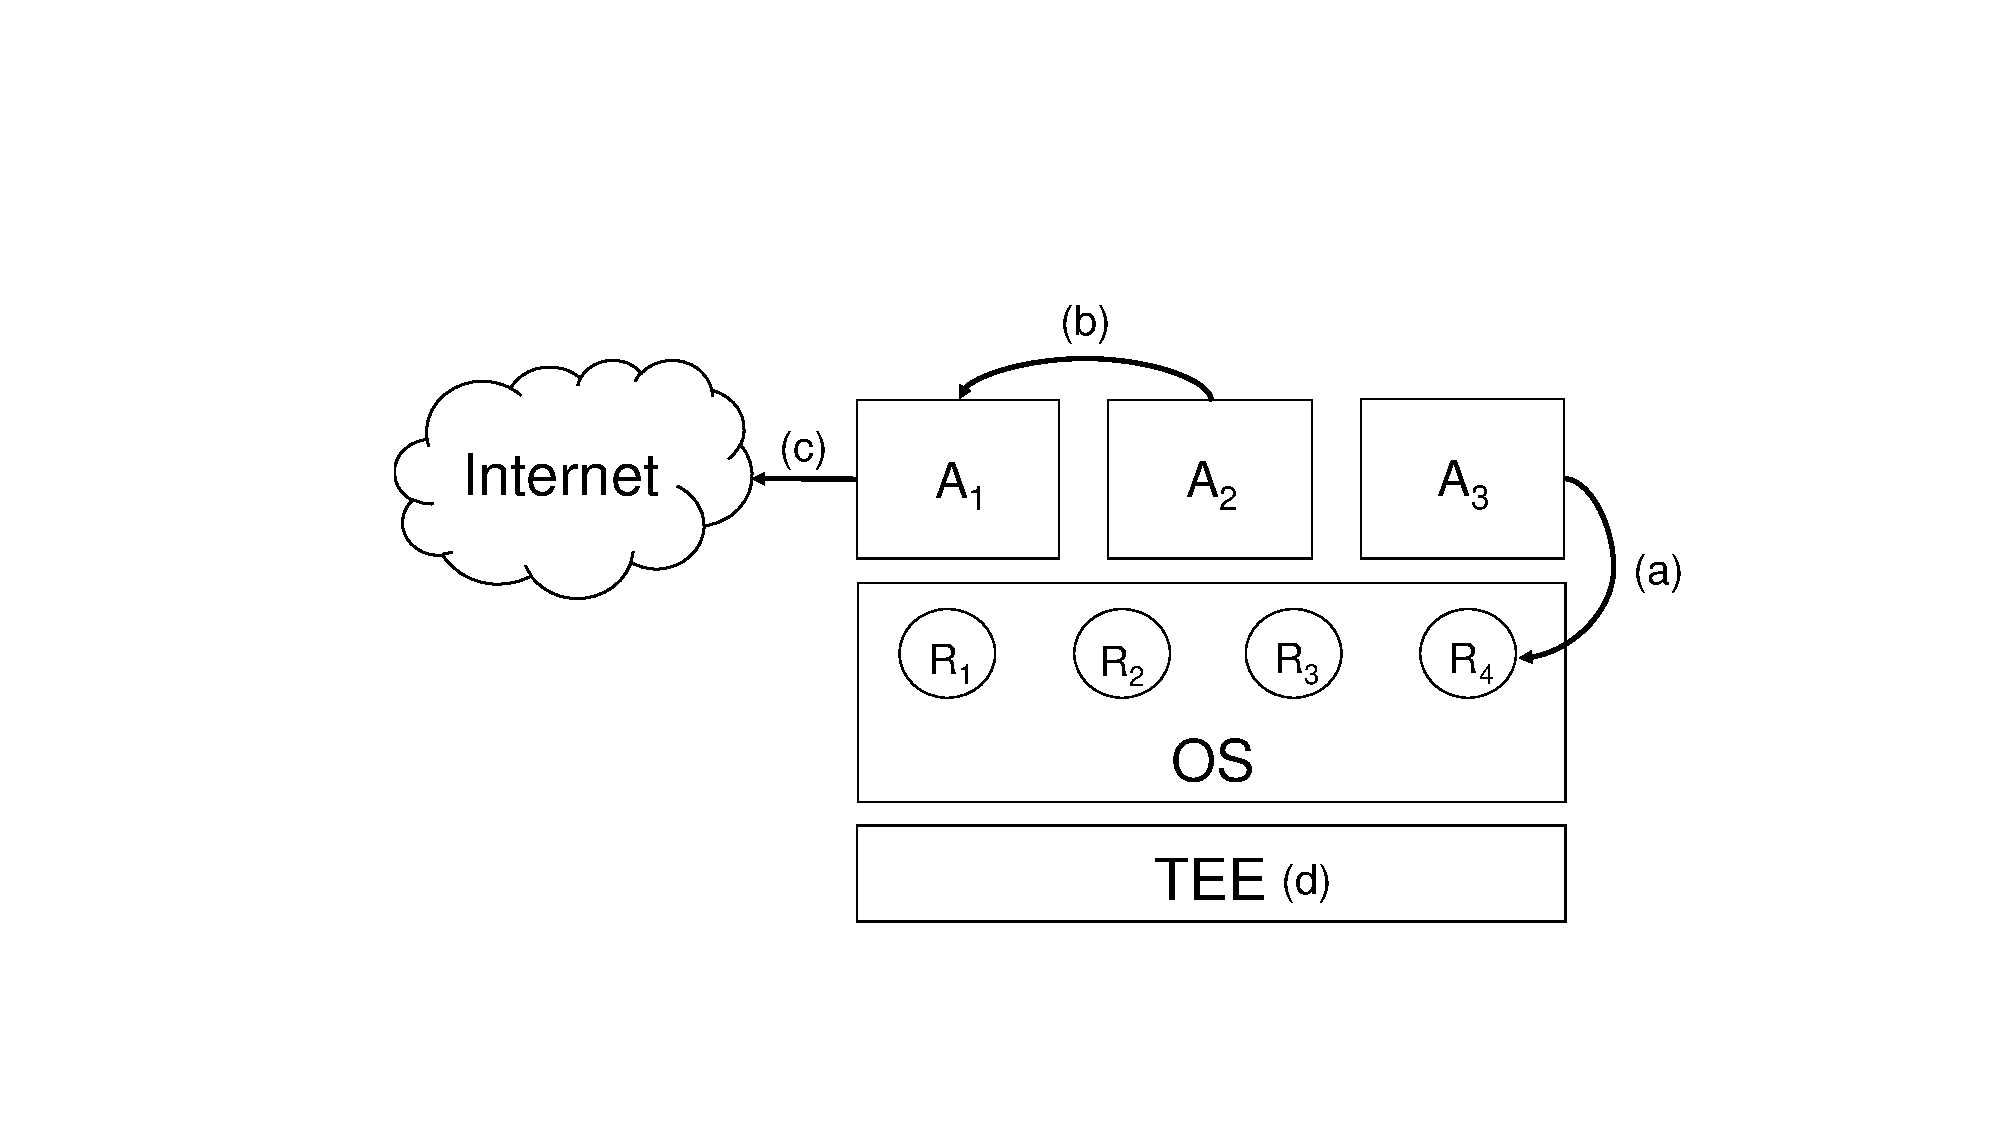
\includegraphics[width=0.65\textwidth]{img/relwork.pdf}
	\caption{Security Mechanisms Map; A-application, R-system resource}
	\label{fig:relwork}
\end{figure}

\subsubsection{Access Control Mechanisms}

%This subsection describes mechanisms and implementations of systems responsible for limiting applications' access to system resources and sensitive data, hence access control mechanisms.

% TENTAR RESUMIR ISTO MAIS UM BOCADINHO?
%Não ponhas em bold-itálico; ao fim e ao cabo, isto é o título da subsecção. ENTAO FAÇO O QUE?
\paragraph{\textbf{Access control mechanisms}} implement security models in which subjects (e.g. user, processes, threads, etc.) are constrained by a security policy to perform certain actions on the system, namely access to resources (e.g. files, sensors, etc.), typically called objects. Android inherits a \ac{DAC} access control mechanism from it's Linux based kernel, but some system resources, such as the IPC Binder mechanism, are accessed via \ac{MAC} policies. In a \ac{DAC} system the data owner is responsible for this data and thus determines who can access it. In Android, an application can create and store files in the filesystem, thus becoming the sole owner of these files, and it can allow access to these files to any other application. In \ac{MAC}, subjects are much more restricted in determining specific permissions because the restrictions on these resource permissions are defined by a global system policy instead. In the Android operating system once a subject attempts to access an object, it triggers a policy evaluation by the kernel, which assesses whether the access may be granted. The advantage of this strict system is its robustness and restrictiveness, because subjects cannot override or modify the security policy. In Android, applications must specify in their manifest the permissions they require at runtime, and after the installation neither applications nor users have any control over the access policies.

Because \ac{MAC} is more restrictive, several systems were created over the years to extend \ac{MAC}'s access control model to other Android resources. SEAndroid~\cite{smalley2013security} solves problems related to resources complying with the \ac{DAC} mechanism. The authors ported SELinux~\cite{peter2001integrating} to provide \ac{MAC} at the kernel layer. The kernel was then modified to support a new \ac{MAC} policy (e.g., filesystem, IPC) and a new middleware layer (MMAC) was created to extend \ac{MAC} to Android's Binder IPC. TrustDroid~\cite{bugiel2011practical} extends the \ac{MAC} mechanism to all the platform's resources in order to isolate different domains' sensitive information.

\paragraph{\textbf{Permission Refinement}} %ISTO TEM QUE SER RESUMIDO MAIS UM POUCO

The Android permission mechanism is a very restricted system. At install time, a list of permissions an application specifies in its manifest file is shown to the user, which is forced into a binary decision, either granting all permissions or quitting the installation. Furthermore, some of these applications may even require more permissions than those effectively needed. This is an inflexible solution, which makes it impossible for users to have full control of the permissions an application effectively requires at runtime. This inflexibility allows apps to use the device's resources whenever the app wishes without the user's knowledge, possibly with malicious intent.

Over the years, many systems aimed at improving the state of affairs through permission refinement. APEX~\cite{nauman2010apex} modified Android's permission model to allow users to specify the assignment of permissions to each app, both at install and runtime. Permission Tracker~\cite{kern2012permission} allows users to be informed on how the permissions are used at runtime and offers the possibility of revoking these permissions. Furthermore, a user can specify which permissions are of interest so they can be notified of every permission access and decide whether to grant or deny that access. These systems improve upon the original Android permission model, but require manual configuration by the user. % tempo verbal no they
A more useful solution would be to use a context-aware system to handle the permissions at runtime. This way it may be possible to, without manual configuration, restrict permissions to all applications running along side a security sensitive app, thus isolating this application and avoiding possible leaks by shared resources.

There are several context-aware permission refinement systems developed by the research community. Trusted third parties can use CRePE~\cite{conti2011crepe} to enforce security policies on another devices. For example, an employer may enforce a security policy on the employees' mobile devices when inside the company, in order to protect the company's interest. Similarly, MOSES~\cite{russello2012moses} enforces domain isolation through the concept of security profiles, allowing it to switch security profiles based on pre-established conditions (e.g., GPS coordinates and time). Additionally, MOSES leverages TaintDroid~\cite{enck2014taintdroid} to prevent apps from one profile to access data belonging to another. Both CRePE and MOSES suffer from a device control issue where a third party defines a policy that cannot be revoked by the user. Moreover, a user has no way to deny the enforcement of a third party policy. 

\paragraph{\textbf{Access Control Hook APIs}}

Most security extensions, such as CRePE~\cite{conti2011crepe} or MOSES~\cite{russello2012moses}, require modifying and adding components to the kernel and middleware layers in order to implement new security models. Some frameworks, such as \ac{ASM}~\cite{heuser2014asm} and \ac{ASF}~\cite{backes2014android}, have been built by the research community in order to ease this development process. These frameworks allow developers to easily create new security models as ordinary Android applications whilst benefiting from a full callback system, which allows these apps to be notified of accesses to resources of interest.

These frameworks comprise a set of hooks distributed among the kernel and middleware layers, which can be registered by a secure application. When a hook is activated it triggers a callback from the Hook API module, which in turn is forwarded to the app for verification. The app then decides if the operation that triggered the activation of the hook may or may not proceed. The main advantage of these frameworks is the flexibility and freedom given to developers in choosing whatever resources to manage.

\paragraph{\textbf{Memory Instrumentation}}

Memory instrumentation leverages application code analysis techniques to restrict access from those applications to the corresponding resources, thus can be used as an access control mechanism. Memory instrumentation can be divided in two groups: static memory instrumentation and dynamic memory instrumentation. While static memory instrumentation changes already compiled bytecode, dynamic instrumentation patches running processes, and for this reason it supports the enforcement of new security models. DeepDroid~\cite{wang2015deepdroid} relies on dynamic memory instrumentation to enforce fine-grained context-aware security policies for enterprise and does this by patching several system services and tracing system calls to resources of interest.

\paragraph{\textbf{Digital Rights Management}} is a specific access control technology which allows data owners to restrict if and how their data can be copied and also how it can be handled once transferred to another device. The \ac{DRM} ecosystem is composed of the following entities:

\begin{itemize}
	\item \emph{User} - human user of the DRM Content
	\item \emph{Content Issuer} - entity that delivers the content
	\item \emph{Rights Issuer} - entity responsible for assigning permissions and constraints to \ac{DRM} content
	\item \emph{Rights Object} - XML document generated by a Rights Issuer expressing the restrictions associated to the content.
	\item \emph{\ac{DRM} Agent} - trusted entity responsible for enforcing permissions and constraints upon the \ac{DRM} content
\end{itemize}

The \ac{OMA} developed a DRM standard~\cite{drm} which defines the format of the content delivered to DRM Agents, as well as the way this content can be transferred from the Content Issuer to the DRM Agent. Android provides an extensible DRM framework, called Android DRM Framework~\footnote{http://developer.android.com/reference/android/drm/package-summary.html}, allowing application developers to enable their apps to manage rights-protected content by complying with one of the supported DRM schemes (specific mechanisms, enforced by DRM Agents, to handle particular types of files).

To understand how \ac{DRM} works in the context of mHealth one can suggest the simple example of a \ac{PHR} mobile health application. In this scenario, the healthcare provider (e.g. a hospital) would be the \emph{content issuer}, and it would use a \emph{rights issuer} to assign the restrictions imposed upon the \ac{DRM} content, which in this case would be the personal health record of a patient, when this content is transferred to the patient's device. When using \ac{DRM}, the patient is limited to access the content through a \emph{\ac{DRM} Agent}. Although this solution seems to fit the security properties a critical applications requires, once again the whole operating system is considered as trusted computing base, and resources shared by different applications such as the framebuffers and display devices may leak sensitive information if the system would become compromised.

\subsubsection{Application Communication Monitoring}

\begin{figure}[t!]
	\centering
	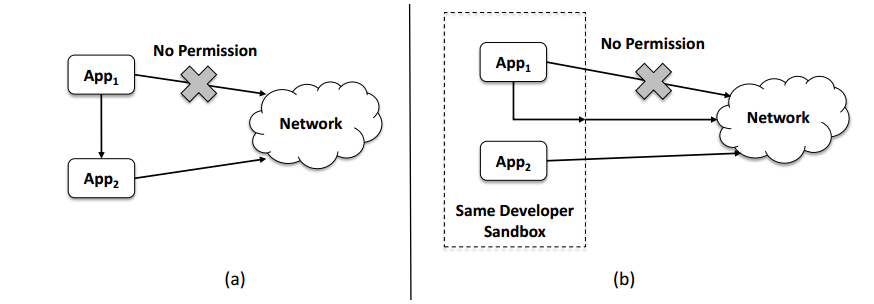
\includegraphics[width=0.95\textwidth]{img/communicationattacks.png}
	\caption{Confused deputy attack (a); Collusion attack (b) - (taken from Duarte \cite{nunoduarte})}
	\label{fig:communicationattacks}
\end{figure}

The Android operating system implements a middleware mechanism called Inter-Process Communication (IPC) which allows different processes, i.e. applications, to communicate between each other and controls how apps access system components and other apps. But this mechanism can be abused such that applications access unauthorized resources or data. In this section we describe two attacks based on Android's IPC mechanism followed by systems developed to mitigate such attacks. The attacks described are called \emph{Confused Deputy Attacks} and \emph{Collusion Attacks} and are represented in Figure~\ref{fig:communicationattacks}.

Confused deputy attacks basically consist of unprivileged applications taking advantage of other applications’ publicly accessible APIs to perform an unauthorized action. If App 2 publicly allows other apps to use the Internet though its API, then the user is unaware that App 1 can use the Internet without explicitly requesting it in Android's manifest. Collusion attacks consist of an app, which might not have permission to perform an operation, still being able to perform it if there exists another app, belonging to the same developer, installed on the user’s device with the permission to perform said operation. This happens because Android’s permission system is based on UIDs.

Confused deputy attacks allow applications to use resources without explicitly specifying the necessary permission to do so, and to mitigate such attacks the research community developed Saint~\cite{ongtang2012semantically} and QUIRE~\cite{dietz2011quire}. Saint was created to specify which apps can access the public APIs of another app. Other systems control this by extending Android’s \ac{IPC} mechanism. QUIRE denies access to an API if in the message exchanged between apps, which contains the full call chain context, the source of the request does not have the necessary permission to access the corresponding data.

Collusion attacks are based on a malicious developer building a legitimate application and persuading the user to install a second app with different permissions. Both apps can collude to leak sensitive information by cooperating with each other. XManDroid~\cite{bugiel2011xmandroid} extends the Android permission model in order to support policies that could constrain the way apps interact with each other. This system prevents data leakage or other types of collusion attacks by developing a graph at runtime with a representation of the apps’ interactions, which is then used to regulate app inter-communication.

\subsubsection{Privacy Enhancement Systems}

The biggest concern for privacy-sensitive mobile applications is sensitive data leakage, specially with valuable data such as health records or banking information. In this section we describe systems which control the flow of sensitive information in order to assess whether such information leaves the systems unintentionally, consequence of a malicious action. Systems like MockDroid~\cite{beresford2011mockdroid} and Zhou et al.~\cite{zhou2011taming} are extensions to Android's data access control mechanism and prevent untrusted applications from accessing sensitive data by allowing users to manually specify application access rights over the system services, such as geographic location.

Other systems, like IdentiDroid~\cite{shebaro2014identidroid} focus on protecting the identity of the user. This is done by using an anonymous mobile device state to provide data shadowing~\footnote{Data shadow is the return of empty or incorrect information instead of the intended data.} and permission revocation techniques that disable the ability of apps to use system services such as location or \ac{IMEI}. This way, if an app is trying to use the device's location, a default location is returned instead of the real one or the application simply cannot access the location service.

Some systems use a different approach to solve the sensitive data disclosure problem. Unlike data access control mechanisms, dynamic taint analysis systems, such as TaintDroid~\cite{enck2014taintdroid}, prevent data leakage by tainting data with a specific mark and then evaluate how this data is propagated through the system. If this data attempts to leave the system the user is alerted. This system suffers from limitations such as \emph{(i)} tracking a low number of data sources (mainly sensors), \emph{(ii)} performance overheads not tolerable for most mobile environments, \emph{(iii)} the existence of false positives leading to access control circumvention and \emph{(iv)} the incapacity of analysing sensitive information leakage through covert channels.
%Existem mais sistemas baseados no taindroid para fazer isto. Podes adicionar uma frase que os cita.

Although these systems can be leveraged in order to understand if sensitive data is leaving the system through network sinks, they fall short in isolating an environment for users to securely input data to the system, meaning that a malicious OS may log user keystrokes and disclose sensitive input data. Furthermore, these systems are not prepared to assess whether data is accessed via shared resources such as framebuffers and display devices, meaning that a compromised OS may access such resources and disclose sensitive information.

\subsubsection{Trusted Execution Systems}
\label{sec:tee}

%Faz melhor a ligação para se perceber porque estiveste a falar de privacy systems e agora de trusted execution. Relaciona isso com o teu objectivo final que é implementar canais de output seguros para as aplicações móveis.
All of previously discussed systems fail at isolating the execution environment for critical mobile applications, and because of this the trusted computing base includes the full-featured operating system responsible for the apps execution. Trusted execution systems disable specific software components of the system and ensure that sensitive application code and data are loaded into a restricted execution environment, thus reducing the trusted computing base.

\paragraph{\textbf{TrUbi}} is a system, developed by Duarte \cite{nunoduarte} and Costa \cite{miguelcosta}, built on top of ASM \cite{heuser2014asm} which allows for flexible system-wide resource restriction. This system may be used to isolate privacy-sensitive apps by killing, freezing or revoking permissions to running applications. With TrUbi it is possible to isolate the execution of a critical application from the remaining apps installed on the system, for example, a simple \ac{PHR} app to display, manage and store personal health records could be developed with the following premise. When the \ac{PHR} app is running, all the other apps are killed and all the resources blocked. The app could then download the health records from the healthcare provider and show the data to the user. When the user exits the application, their data is encrypted with a key generated from a user password, and only then the resources are released for the other applications. The system was completely isolated during the whole process and the data is stored with encryption (and the key, because it is generated from a user password, is not stored on the system).

Although TrUbi effectively reduces the TCB dynamically by disabling concurrent running processes, it still trusted the operating system's code base which may be compromised by malware. Furthermore, TrUbi has no support for trusted UI meaning that a compromised OS can access sensitive data by disclosing the content of resources such as graphical framebuffers and display devices. The following systems allow for a more significant reduction of the trusted computing base by isolating the execution environment of sensitive code from that of a full-featured operating system.

\paragraph{\textbf{External hardware security modules}} represent the classic security solution for embedded applications, which is the inclusion of a dedicated trusted element (e.g., a smartcard) that is outside of the main \ac{SoC}. On one hand, the main advantage of this solution is that it allows for the encapsulation of sensitive assets inside a physical device specially designed for robust security. On the other hand, the main disadvantage is that smartcards provide only secure processing and storage functions. This means that some operations (e.g., I/O) must rely on software running outside of the security perimeter to provide the desired features. An example where this happens is when a user interacts with the system by entering a \ac{PIN}. This \ac{PIN} must be managed by the less secure software outside of the smartcard, making it vulnerable to attacks. Meaning that, although this security solution does not trust the code base of a full-featured OS to achieve its goals, it requires some untrusted interaction with the rich OS in order to offer additional features such as content display, which cannot be trusted as it relies on information received from the untrusted rich OS.

\paragraph{\textbf{Internal hardware security modules}} are, contrary to the previous solution, included within the \ac{SoC}. These integrated modules are usually one of two forms: the first is a hardware block designed specifically for managing cryptographic operations and key storage, and the second is a general purpose processing engine, which is placed alongside the main processor, that uses custom hardware logic to prevent unauthorized access to sensitive resources. This solution has the advantage of being cheaper and offering a performance improvement over external hardware security modules like smartcards. The disadvantage is that, like the previous solution, the resources protected by the security module will eventually need to be used outside the module it self, thus making these resources vulnerable. Another disadvantage is that this design requires a separate physical processor, typically less powerful than the main processor, to a avoid sharing such an important resource with less critical modules.
% TODO ENTREGA - como assim?
% Dá um exemplo de um recurso controlado para se perceber melhor do que estás a falar

Because both the external and internal hardware security modules require the sensitive content to eventually be used outside the isolated environment, for instance for display purposes, there is still the need to eventually trust in the OS to support additional features. The next systems solve this problem by allowing complete isolation between different execution environments.

\paragraph{\textbf{Software virtualization}} is a software security mechanism with a highly trusted management layer called hypervisor, which runs in privileged mode of a general purpose processor. The hypervisor uses a \ac{MMU} to separate several independent software platforms, running each one inside a virtual machine. There are many advantages of using this solution. The first advantage is that a compact hypervisor can be thoroughly tested to ensure, with a high degree of certainty, that software running within one virtual machine cannot influence and attack the execution of others running in parallel. Another advantage is that there is no additional hardware requirement to implement a hypervisor, thus any processor with a \ac{MMU} can be used to implement this security solution. Lastly, this solution supports processing isolation between a secure environment and a full-blown rich operating system running in different virtual machines managed by the hypervisor. If a communication mechanisms is supported by the hypervisor, then a secure pipeline can be established between the two virtual machines.
% Tens que citar alguma coisa aqui.
%TODO ENTREGA
% NAO TENHO O QUE CITA, ISTO FOI TIRADO DO WHITEPAPER DA ARM TRUSTZONE
The main disadvantage with this approach is that having another software component managing resources, such as GPUs, have a high impact on system performance. For this reason a new hardware architecture was designed to offer the benefits of software virtualization without the disadvantages of running additional software components.

\paragraph{\textbf{TrustZone}} is a hardware architecture that extends the security throughout the system's design. This architecture was designed to allow for the execution of an isolated small kernel inside trusted hardware. With this architecture, the sensitive data can be completely isolated for the full-features operating system and trusted applications can execute without relying on large and complex code bases, thus enabling end-to-end security without exposing resources to an untrusted system. TrustZone also mitigates performance overheads inherent to software virtualization techniques since the hypervisor mechanism, which manages the trusted and untrusted domains, is implemented natively in hardware.

\begin{figure}[t!]
	\centering
	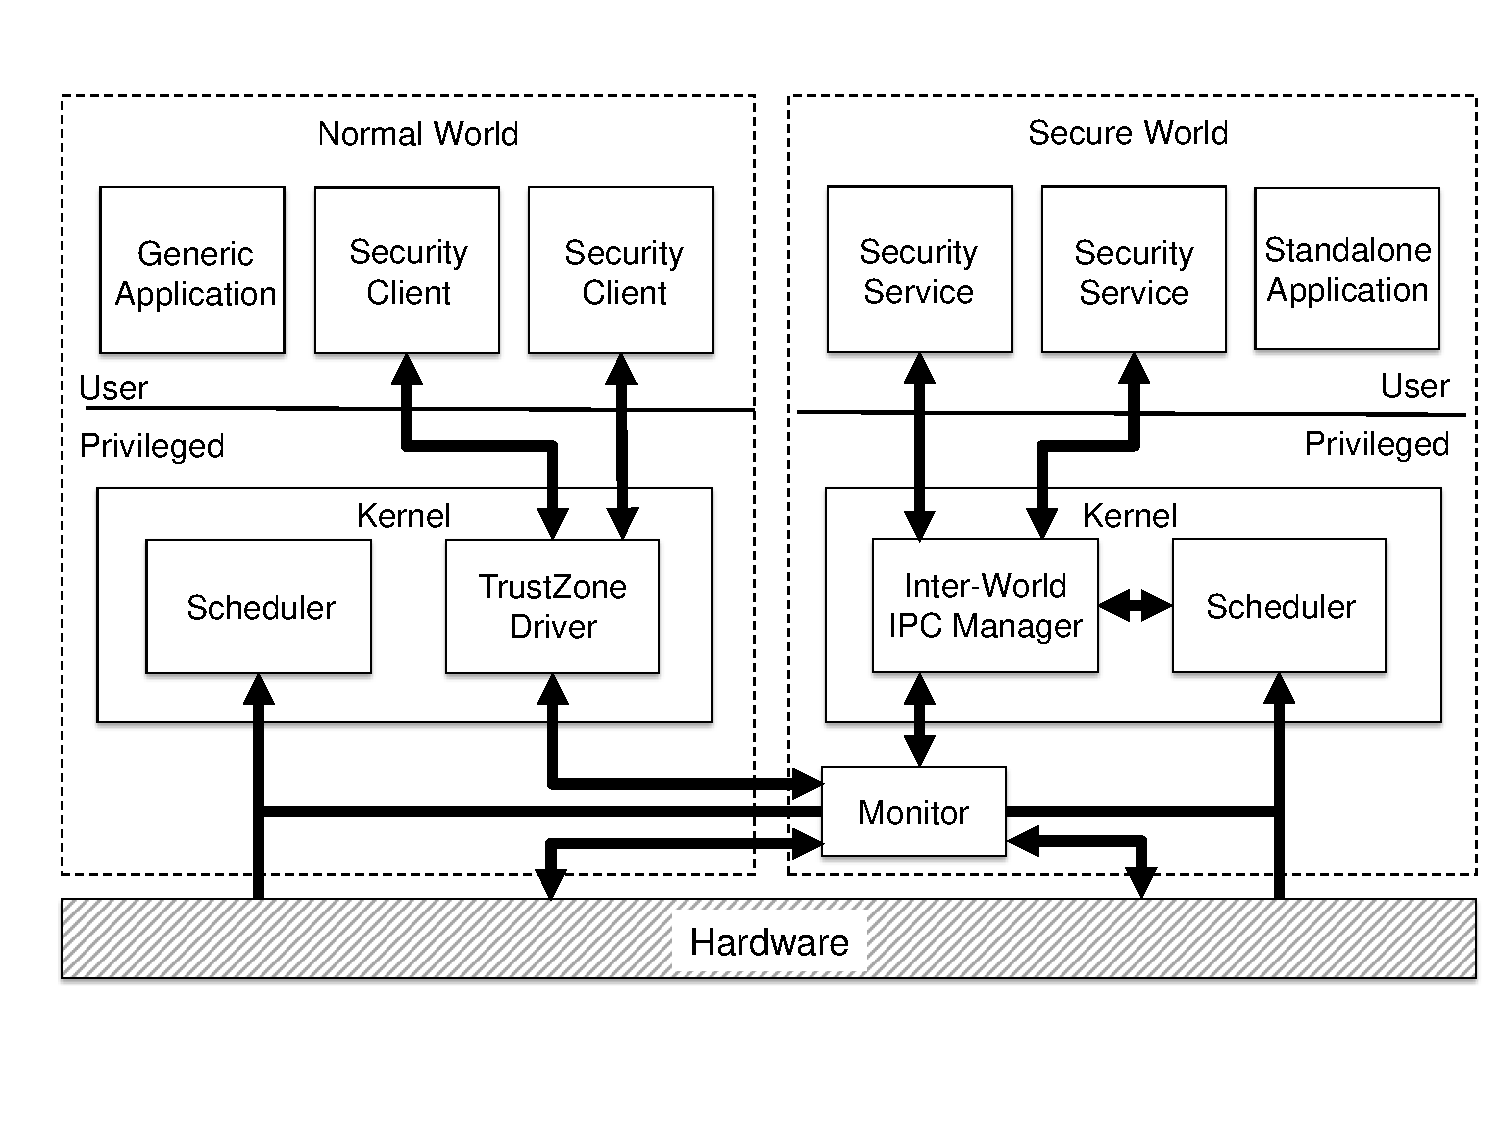
\includegraphics[width=0.80\textwidth]{img/trustzone.pdf}
	\caption{TrustZone's Software Architecture (adapted from \cite{trustzone_whitepaper})}
	\label{fig:trustzone_architecture}
\end{figure}

TrustZone hardware and software architecture are described in a whitepaper~\cite{trustzone_whitepaper} by ARM. In a TrustZone-enabled system, a physical processor provides two virtual cores, one considered non-secure and the other secure, as well as a robust context switching mechanism known as monitor mode. The NS bit sent on the main system bus identifies which of the virtual core performed an instruction or data access. Several software architectures can be implemented on the software stack of a TrustZone-enabled processor, but the most powerful one is a dedicated operating system in the secure world, as shown in Figure~\ref{fig:trustzone_architecture}. This design allows for concurrent execution of multiple secure world applications and services that are completely independent from the normal world environment, thus even with a compromised normal world the secure world executes as expected. Moreover, if the secure world kernel is small and correctly implemented, security applications can execute at the same time without needing to trust each other. The kernel design can enforce the logical isolation of secure tasks from each other, preventing one secure task from tampering with the memory space of another.

\subsubsection{Summary}

After describing the state of the art of general-purpose mobile security mechanism, we discuss which systems have the potential to support the development of critical security applications with embedded secure displays and inputs in insecure mobile interfaces.

Access control mechanisms focus on restricting access to system resources, which may be useful for critical applications if these can use it to limit the access of less sensitive applications to shared resources whilst they are running. But these mechanisms rely on a full-blown operating system, with a large and complex TCB, to ensure this property, which may become compromised by malware and intentionally sabotage these security measures. Moreover, these systems do not offer trusted user interfaces as they provide no explicit isolation between the operating system and the critical application handling sensitive data, i.e., resources such as display devices and framebuffers are shared between both the OS and critical application, which may lead to data leakage if the OS becomes compromised. For these reasons, access control mechanisms do not fulfil the needs of this project.

Application communication monitoring focuses on assuring that communication attacks cannot effectively target Android's IPC mechanism, which is the main communication component between applications in the Android platform. Because these systems are not meat to be used for the development of applications, but rather as a protective measure against specific attacks, these mechanisms are not suitable to solve the underlying problem of developing critical applications to securely display, manage and store sensitive data.

Privacy enhancement systems focus assessing whether sensitive data leaves the system via network sinks. While these systems are useful in controlling the data flow of traditional paths, such as Android's IPC, it falls short of controlling the data flow of unconventional paths, such as framebuffers and display devices, meaning that sensitive data may be intercepted by a malicious OS without the privacy enhancement system knowing it. Furthermore, these systems do not offer any secure input feature, which is understandable as this is not its goal.

Trusted execution environments focus on supporting an isolated environment which comprises a smaller TCB than that of a full-featured operating system. This category comprises very different systems with different purposes and approaches, which we summarize next. TrUbi dynamically reduces the overall system's TCB while a critical application is runnning, but this is done whilst relying on the operating system, meaning that a compromised OS may compromise the systems execution.

External and internal hardware security modules offer an isolated hardware-based environment for the execution of secure tasks. But because both external and internal modules provide only secure processing and storage functions, the data it protects must eventually be used outside the isolated environment, for instance for display purposes. This means that these systems still rely on the untrusted OS for functionality such as trusted UI, which we want to be supported by the secure environment.

Software virtualization leverages a trusted software layer called hypervisor which supports total isolation between execution environments by running each system inside a virtual machine. In addition, because this software layer manages all system resources, instead of the rich OS, it can securely support trusted user interfaces because sensitive data never reaches the untrusted domain if the hypervisor clears the shared resources before hand. The main disadvantage of this approach is the performance overhead of having another software component managing resources, which greatly hinders the overall performance.

Lastly, TrustZone also supports trusted user interfaces by controlling the necessary peripherals and also supports isolated environments running along side one another. But, unlike software virtualization, TrustZone leverages special purpose hardware to isolate both domains, which mitigates the performance overhead problem. For this reason, TrustZone will be discussed in depth in the next section, as it supports all the features necessary to implement \emph{ViewZone}. 

%After describing and assessing the available technology, one can argue which mechanisms better suit the development of critical mobile applications for Android, such as our \ac{PHR} app. Access control mechanisms and application communication monitoring systems are clearly unsuitable for the goals of this project.
%%Aqui, é preciso focar claramente no objectivo do teu projecto: (1) suportar um mechanismo de trusted output, e (2) ter pequena TCB.
%These systems may be helpful in developing new access control policies or mitigating vulnerabilities caused by negligent development, but are not sufficient to build privacy-sensitive applications. % porquê?
%Privacy enhancement systems focus on detecting and preventing data leakage instead of providing a framework for developers to build privacy-sensitive applications, for this reason these systems do not fulfil the needs of this project. % muito vago. Mais claro.
%Besides the problems discussed above, all these mechanisms suffer from a critical limitation, both the middleware and the underlying kernel are considered as trusted computing base. This means that if a malicious app is capable of compromising these layers, then a critical application is compromised as well, and the data it protects may be accessible by a malicious party. The only solution for the problem described is using a \ac{TEE}. % vago
%%As shown in table~\ref{tab:securityMechanismsComparison}, the \ac{TEE} solutions are the only solutions which work either with a trusted OS and a compromised OS.
%
%To accomplish the goals of this project, a completely secure flow of execution is needed, this means that privacy-sensitive data must never leave the trusted security perimeter. %o que é o trusted security perimeter? dizer que é para nao fazer o leakage
%A system which does not support secure I/O greatly limits the functionality offered by a \ac{PHR} application, to the point where it becomes useless. For this reason, both the external and internal hardware security modules were discarded. On a different note, the virtualization solution seems promising, but with all the problems related to sharing resources such as \ac{GPUs} and other system buses, and because total isolation is needed, which is not easily achievable using virtualization by it self, this security module is not appropriate for this project. TrustZone technology seems to be the most complete system of all the \ac{TEE} solutions, as it mitigates recurring problems from other mechanisms. For this reason, the next section will focus on describing some state-of-the-art TrustZone-based systems, as it is the only security mechanism suitable for the needs of this project.

%% Please add the following required packages to your document preamble:
%% \usepackage{graphicx}
%\begin{table}[t!]
%	\centering
%	\caption{Comparison between security mechanisms with and without a compromised Operating System (Android).}
%	\label{tab:securityMechanismsComparison}
%	\resizebox{\textwidth}{!}{%
%		\begin{tabular}{|P{5cm}||P{2.3cm}|P{2.3cm}|P{2.3cm}|P{2.3cm}|}
%			\hline
%			\multirow{2}{*}{Security Mechanism} & \multicolumn{2}{c|}{Correct OS}  & \multicolumn{2}{c|}{Compromised OS} \\ \cline{2-5}
%			& Confidentiality & Data Integrity & Confidentiality & Data Integrity    \\ \hline \hline
%			Access Control Mechanisms			& \cmark 		  & \cmark         & \xmark          & \xmark            \\ \hline
%			App Communication Monitoring    	& \xmark          & \xmark         & \xmark          & \xmark            \\ \hline
%			Privacy Enhancement Systems         & \cmark          & \cmark         & \xmark          & \xmark            \\ \hline
%			Digital Rights Management           & \cmark          & \cmark         & \xmark          & \xmark            \\ \hline
%			TrUbi					            & \cmark          & \cmark         & \xmark          & \xmark            \\ \hline
%			External Hardware Security	        & \cmark          & \cmark         & \cmark          & \cmark            \\ \hline
%			Internal Hardware Security	        & \cmark          & \cmark         & \cmark          & \cmark            \\ \hline
%			Software Virtualization		        & \cmark          & \cmark         & \cmark          & \cmark            \\ \hline
%			TrustZone        					& \cmark          & \cmark         & \cmark          & \cmark            \\ \hline
%		\end{tabular}
%	}
%\end{table}
% Confesso que não sei bem a que te referes com confidentiality e integrity; estes sistemas são muito diferentes uns dos outros...

% TRUSTZONE
\subsection{TrustZone-based Mobile Security Systems}

The research community has been experimenting with hardware security architectures in order to achieve better solutions for common security problems, such as two-factor authentication or cryptographic key generation. Among the available security architectures there is ARM's TrustZone technology, a trusted hardware which allows the development of a diverse set of security systems and services, such as Samnsung KNOX and DroidVault. TrustZone is becoming popular as it support code to be executed isolated from a full-featured operating system such as Android. This allows for a reduced trusted computing base on the critical applications running in the isolated environment.

One of the most important uses of TrustZone is for building trusted execution environments (TEE), which are compact systems running in the secure world of the TrustZone hardware in order to provide and isolated environment for critical applications. Since its formal standardization by the OMTP in 2007, several \ac{TEE} software stack architectures have been implemented. This standard comprises a set of security requirements on functionality a TEE should support. The GlobalPlatform~\footnote{https://www.globalplatform.org/} organization went a step further by defining standard APIs: on the one hand, the TEE internal APIs that a trusted application can rely on, and on the other hand, the communication interfaces that rich OS software can use to interact with its trusted applications. It is worth noting that, because the TEE threat model assumes that nothing coming from the rich OS is trustworthy, the designer of a trusted application must assume that the rich OS side client of the trusted application may not be legitimate.

When surveying the literature, TrustZone-based systems can be divided in two separate groups: Trusted Kernels, and special-purpose Trusted Services. Trusted Kernels allow the execution of generic code in the secure world environment, whilst a Trusted Service implements a specific application in the secure domain. With a more thorough analysis, one can divide each of these categories even further, with regards to trusted user interface (UI). A TrustZone-based system features Trusted UI capability if it allows secure world components to directly access the mobile interface without interference from the rich OS, thus minimizing the risk of, for instance, password logging.

For this reason, this section categorizes TrustZone-enabled systems into four subsections: \emph{(i)} Trusted Kernels with Untrusted UI, \emph{(ii)} Trusted Services with Untrusted UI, \emph{(iii)} Trusted Kernels with Trusted UI and \emph{(iv)} Trusted Services with Trusted UI. Table~\ref{tab:trustzonesystemscomparison} categorizes the systems described in the following subsections.

% TODO ENTREGA
% Não me chocaria se dissesses à partida em que quadrante encaixarias o sistema que queres conceber e porquê.

\begin{table}[t!]
	\caption{TrustZone-based system categorization.}
	\label{tab:trustzonesystemscomparison}
	\centering
	%\resizebox{\textwidth}{!}{%
	\begin{tabular}{ c|c|c| }
		\multicolumn{1}{c}{} 	& \multicolumn{1}{c}{Untrusted UI} 	& \multicolumn{1}{c}{Trusted UI} \\ \cline{2-3}
		\multirow{5}{*}{TAs} 	&									& \\
		& Android Key Store					& TrustOTP \\
		& DroidVault 						& TrustDump \\
		& Brasser et al.					& AdAttester \\
		& 									& TrustUI \\
		&									& \\
		\cline{2-3}
		\multirow{5}{*}{GPFR}	&									& \\
		& TLK								& Genode \\
		& OP-TEE 							& T6 \\
		& Andix OS							& TrustICE \\
		& Nokia ObC							& SierraTEE \\
		& TLR 								& Samsung KNOX \\
		&									& \\
		\cline{2-3}
	\end{tabular}
	%}
\end{table}

\subsubsection{Trusted Kernels with Untrusted UI}

Trusted Kernels have the goal of executing generic code in its isolated environment, and most of theses kernels have similar architectures (similar to the one shown in section~\ref{sec:tee}). This architecture is generally composed of a small trusted kernel running in the isolated secure world of TrustZone-enabled processors, a normal world user space client API and a kernel TEE device driver, used to communicate between worlds.

OP-TEE~\footnote{https://wiki.linaro.org/WorkingGroups/Security/OP-TEE}, TLK\footnote{http://www.w3.org/2012/webcrypto/webcrypto-next-workshop/papers/webcrypto2014\_submission\_25.pdf}, TLR~\cite{santos2011trusted} and AndixOS~\cite{fitzekandix} are \ac{TEE} implementations which share this general architecture. On-board Credentials (ObC)~\cite{kostiainen2012board} is another \ac{TEE} system, originally developed for Nokia mobile devices using the TI M-Shield technology and later ported to ARM's TrustZone, which supports the development of secure credential and authentication mechanisms. Although these systems use TrustZone hardware based isolation to ensure that applications running inside the secure world are not tempered with by a compromised rich OS, they were implemented with the goal of reducing the \ac{TCB} in order to ensure a less vulnerable system, and for this reason there are some limitations regarding the features they can support.

%TODO ENTREGA
% Estes sistemas não têm publicações associadas?
A reduced \ac{TCB} means that most features of standard mobile operating systems are not supported, for instance, in both TLR and OP-TEE, as well as AndixOS, the secure world kernel lacks drivers for peripherals such as the touchscreen or code to control the framebuffer, thus it is not capable of supporting trusted UI. For this reason, these systems do not allow developers to easily build trusted applications for sensitive data display and management. Instead, these sytems support an RPC-like mechanism for in-between-world communication, secure persistence storage and basic cryptographic systems allowing for the development of simple trusted services.

\subsubsection{Trusted Services with Untrusted UI}

As opposed to Trusted Kernels, which enable the execution of general-purpose application code on the secure world, Trusted Services are designed to implement specific applications from the secure world natively. This subsection describes trusted services which do not support trusted UI, or trusted services which do not require trusted UI to correctly perform its function. Some trusted services, such as DroidVault and Restricted Spaces, use custom trusted kernels to fully control the underlying hardware and execution environment and design specific security solution which may not be supported by generic trusted kernels.

%REVER PARA FACILITAR A LEITURA
Brasser et al.~\cite{brasserregulating}, which will be referred to as Restricted Spaces for the remainder of this section, similarly to CRePE~\cite{conti2011crepe} and MOSES~\cite{russello2012moses}, allows for third parties (hosts) to regulate how users (guests) use their devices (e.g., manage their devices’ resources), while in a specific space. This system comprises of authentication and communication mechanisms between the guest's secure world and hosts, and remote memory operations, which allow for configuration changes such as uninstall peripheral drivers, either pointing their interfaces to NULL, or by pointing them to dummy drivers that just return error codes. With this, Remote Spaces is capable of securely refine device permissions using a context-aware approach.

DroidVault~\cite{li2014droidvault} introduces the notion of data vault, which is an isolated data protection manager running in the trusted domain for secure file management, as a protective measure for sensitive data on Android mobile devices. To achieve this, DroidVault adopts the memory manager and interrupt handler from Open Virtualization's SierraTEE~\footnote{http://www.openvirtualization.org/} and is implemented with a data protection manager, encryption library and a port of a lightweight SSL/TLS library called PolarSSL~\footnote{https://polarssl.org/}. Much like the trusted application described above, DroidVault supports world switching through software interrupts and secure boot and even inter-world communication. With this Trusted Service a user can download a sensitive file from an authority and securely store it on the device. The sensitive file is encrypted and signed by the data protection manager before it is stored in the untrusted Android OS, in order to save space in the limited storage capacity available in the secure world domain.

Android Key Store~\footnote{http://developer.android.com/training/articles/keystore.html} is another security service in Android. This service allows for cryptographic keys to be stored in a container (keystore), so its extraction from the device becomes difficult and so they can be used for common cryptographic operations. The encryption and decryption of the container is handled by the keystore service, which in turn links with a hardware abstraction layer module called "keymaster". The android open source project (AOSP) provides a sofware implementation of this module called "softkeymaster", but device vendors can offer support for hardware based protected storage when available by using TrustZone.

These Trusted Services do not fulfil the goals of this project as they do not support necessary features such as secure display and input. On the other, DroidVault takes an interesting approach to secure storage each may be an inspiration for the secure storage problem in \emph{ViewZone}.

\subsubsection{Trusted Kernels with Trusted UI}

In this section we describe Trusted Kernels with support for trusted UI. As referenced before, GlobalPlatform defined standard APIs for the communication between the rich OS running in the normal world and the secure OS, but this organization also defined device specifications which TEEs must comply to in order to be certified. Included in these device specifications is a trusted UI clause, meaning that every TEE which complies with GlobalPlatform's device specifications must support trusted UI. 

SierraTEE~\footnote{http://www.openvirtualization.org/}, T6~\footnote{https://www.trustkernel.com/products/tee/t6.html} and Open-TEE~\cite{mcgillion2015open} comply with this standard, and for this reason allow the development of trusted applications with secure user interfaces. Open-TEE's trusted UI feature is being developed by the community as it was not originally supported.The Genode OS Framework~\footnote{http://genode.org/} is a tool kit for building highly secure special-purpose operating systems to be executed in TrustZone-enabled processors. Genode implements a framebuffer and input drivers to be used by the secure kernel, thus trusted applications running on top of Genode-based TEEs can offer trusted user interfaces.

Samsung KNOX~\cite{knox_whitepaper} is a defense-grade mobile security platform which provides strong guarantees for the protection of enterprise data. This security is achieved through several layers of data protections which include secure boot, TrustZone-based integrity measurement architecture (TIMA) and Security Enhancements for Android (SEAndroid~\cite{smalley2013security}, which was already discussed in previous sections). Samsung KNOX offers a product called KNOX Workspace, which is a container designed to separate, isolate, encrypt, and protect work data from attackers. This enterprise-ready solution provides management tools and utilities to meet security needs of enterprises large and small. Workspace provides this separate secure environment within the mobile device, complete with its own home screen, launcher, applications, and widgets.

TrustICE~\cite{sun2015trustice} is an isolation framework to provide isolated computing environments (ICEs) on mobile devices. A lot of similar solutions provide isolated computing environments by allowing code to be executed in the secure world, generally in the form of trusted applications. TrustICE aims at creating ICEs in the normal world domain rather than in the secure world. For this reason, TrustICE's architecture is slightly different from those described before.

Figure~\ref{fig:trustICE_architecture} compares TrustICE's architecture with those of traditional TrustZone TEE's, where trusted applications run inside the secure world domain. TrustICE works by implementing a trusted domain controler (TDC) in the secure world, which is responsible for suspending the execution of the rich OS as well as other ICE's in the system when another ICE is running, thus supporting CPU isolation for running ICE's. For memory isolation a watermarking mechanism is implemented so the rich OS cannot access secure code running in the normal world memory. In order to isolate I/O devices the secure world blocks all unnecessary external interrupts from arriving at the TDC, thus protecting the TDC from being interrupted by malicious devices, the exception being a minimal set of required interrupts to allow trusted UI.

Because these systems support secure display, input and secure storage they are adequate for the development of trusted applications which require sensitive information to be displayed and managed by the user. However, to develop such application is complex because these trusted kernels are not developer friendly and are not build to support applications with this specific goal. For this reason, there is a need to create a trusted system which allows easy development of critical applications for content display and management.

\begin{figure}[t!]
	\centering
	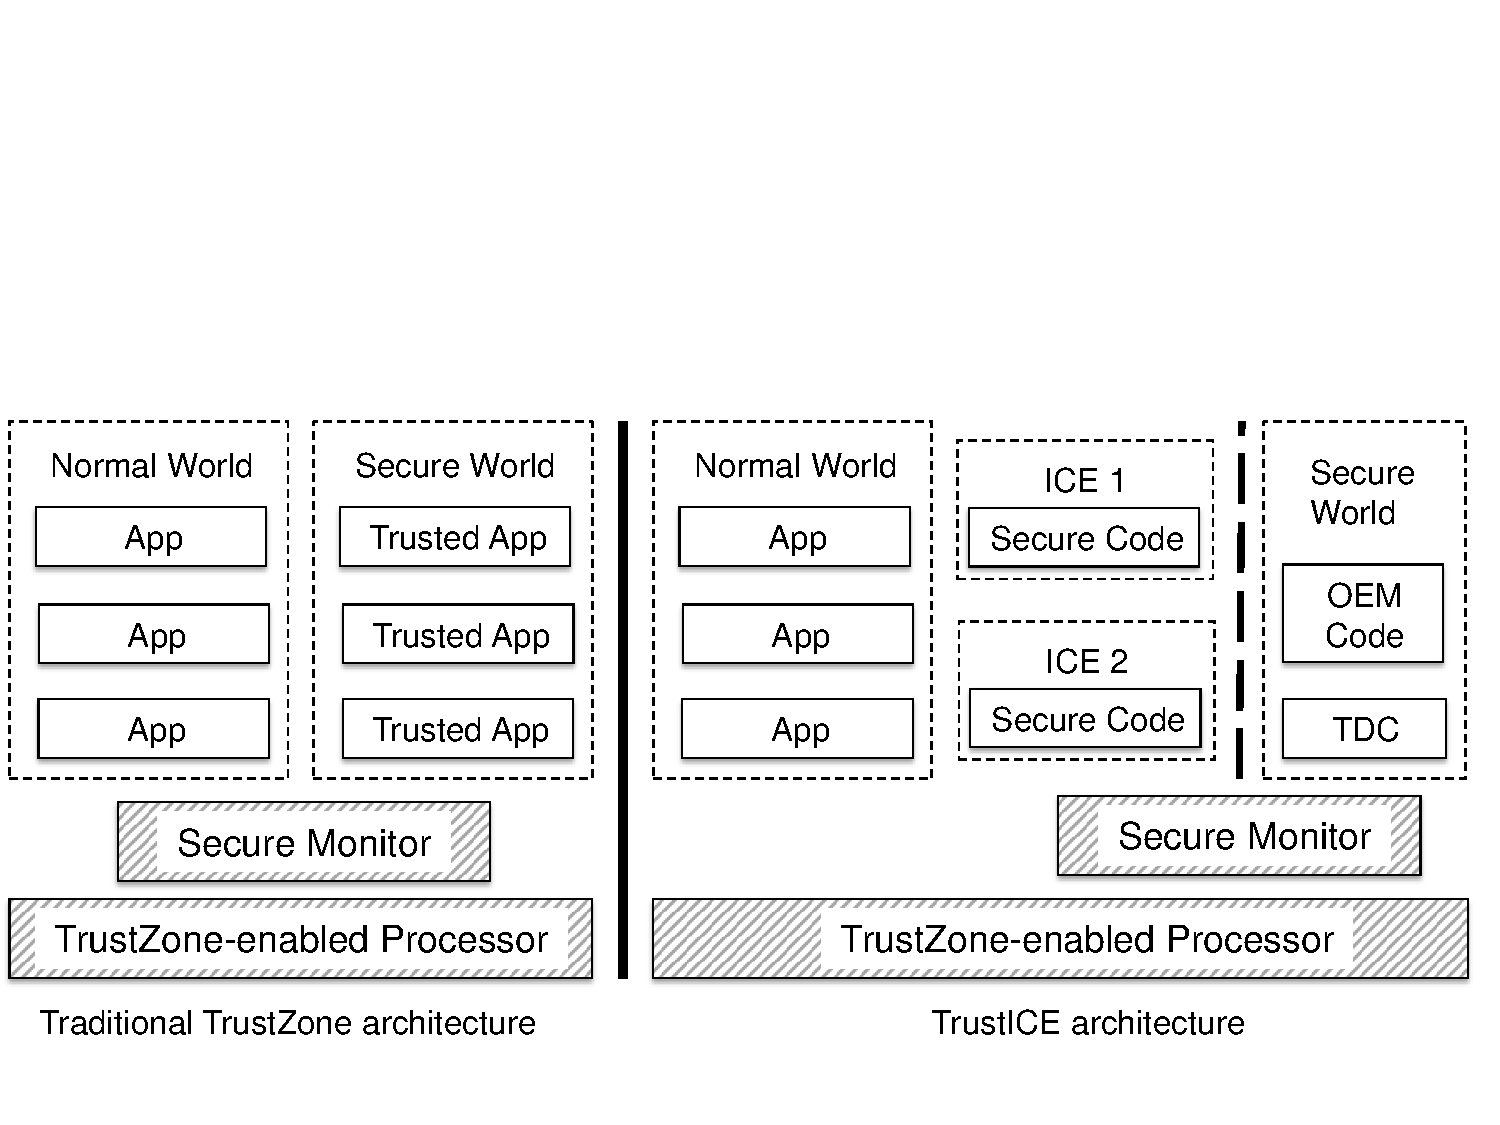
\includegraphics[width=0.80\textwidth]{img/trustICE.pdf}
	\caption{Architecture comparison between traditional TrustZone's software stack and TrustICE (adapted from~\cite{sun2015trustice})}
	\label{fig:trustICE_architecture}
\end{figure}

\subsubsection{Trusted Services with Trusted UI}

Besides Trusted Kernels, some Trusted Services offer secure display and input to the applications implemented secure domain. Usually, this is done by implementing secure touchscreen drivers and secure framebuffers in the secure world, thus isolating the resources which support trusted user interfaces.

TrustOTP~\cite{sun2015trustotp} is a One-Time-Password (OTP) system, secured by hardware, where the OTP is generated based on Time and a Counter secured by TrustZone's memory management. Most trusted applications described before require inter-world communication to trigger the world-switching mechanism. This system leverages hardware interrupts to trigger the world-switch. This mitigates denial-of-service attacks by a malicious rich OS which may control the inter-world communication mechanism and intercept the calls (software interrupts) required to trigger the world-switch. 

TrustDump~\cite{sun2015reliable} is a secure memory acquisition tool and offloads the memory through micro-USB. Simmilarly to TrustOTP, this system relies on hardware interrupts to trigger world-switchs. This solution may be implemented by systems which require no inter-world communication, but for systems which need to offer seamless integration with the normal world this approach may have to be leveraged with other development strategies. Both of these systems support trusted UI by implementing secure display and input drivers and display controllers to manage the secure framebuffers.

Instead of implementing the required drivers to support trusted UI, some systems designed mechanisms to allow the reuse of untrusted drivers, implemented in the rich OS, by the secure world domain.
% Melhorar este parágrafo para se perceber de forma mais clara.
TrustUI~\cite{li2014building} excludes the device drivers for input, display and network from the secure world, and instead reuses the existing drivers from the normal world, thus achieving a much smaller TCB than previously described systems. Because we are only interested in trusted UI, the following explanation discards the network delegation mode. To achieve trusted UI, device drivers are split into two parts: a backend running in the normal world domain and a frontend running in the secure world. Both parts correspond through proxy modules running in both worlds, which communicate via shared memory. Whenever secure display is necessary, the frontend asks for a framebuffer from the backend driver and sets that memory region as secure only, thus isolating the framebuffer from rich OS manipulation. 

Because this mechanism can still be victim of framebuffer overlay attacks, where a malicious backend driver gives a false framebuffer to the secure world, the system randomizes the background and foreground colours used in the display and uses two LEDs, controlled by the secure world, to show these same colours. A user can visually check if the colours shown in the secure LEDs match those of the display. If they match then the user is assured that the display shown is being controlled by the secure world. To support trusted input from the user, TrustUI introduces a randomization mechanism to generate different software keyboards for every input of the user. This means a malicious rich OS cannot correctly intercept user input. But a malicious system still disclose, for instance, the length of a password and for this reason, the keyboard mechanism introduces, from time to time, \emph{confirm} buttons randomly positioned on the screen before continuing. This method also prevents fake key injection attacks, where a malicious system would trick the secure world into believing those key strokes were authentic and originated from a real user.

Because these systems support secure display and secure input they do not disclose sensitive data. However, TrustOTP and TrustDump do not offer a fully integrated environment with the Android running in the normal domain. TrustUI, on the other hand, fully integrates its environment with that of the Android operating system. Furthermore, TrustUI describes a novelty mechanismm for the reuse, by the secure domain, of untrusted driver implemented in the normal world without compromising security, which significantly reduces the secure system's trusted computing base. The main disadvantage of TrustUI is that, similarly to TrustOTP and TrustDump, does not support the development of generic display applications. Besides, TrustUI is not immune to denial-of-service attacks by a malicious operating system running in the normal world, which may compromise the execution of the secure system.
%\cleardoublepage
%%!TEX root = ../report.tex

% 
% Architecture
% 
% (2/3pgs)
\section{Architecture}
\label{sec:architecture}

This section describes \emph{ViewZone}, a novel security framework for TrustZone-enabled devices which supports the development of secure sensitive applications, while leveraging Android as the untrusted rich OS, with the particular purpose of displaying privacy sensitive data to the user. This information may take several formats, either being images, pdfs or straight plain text files. This flexibility allows app developers to easily create several basic secure applications such as a secure password managers, sensitive images display (for instance, for military purpose) and sensitive document managers, without ever being at risk of disclosure by a compromised full-featured operating system. To fully demonstrate the concept of \emph{ViewZone}, we develop a sensitive mobile health application for managing personal health records. The following subsections describe the underlying \emph{ViewZone} system architecture and the purposed \ac{PHR} application.

%% ==== SYSTEM ====
\subsection{ViewZone}

\emph{ViewZone} must maintain a small trusted computing base in order to guarantee a secure foundation for sensitive applications. This means only the strictly necessary features for practical applications to work must be supported, and even these features must be built with intelligent and conservative development strategies. Moreover, \emph{ViewZone} must allow for an integrated environment with Android to provide a transparent isolated security environment for these sensitive applications without compromising the system's usability. To support the described features this project must fulfil the goals of assuring the necessary security policies such as confidentiality, integrity and authenticity of data stored in the untrusted world, must support trusted user interfaces and be developer friendly, which is allow for easy development of simple secure applications such as those described above. The following paragraphs describe how these goals will be supported in \emph{ViewZone}.

\paragraph{\textbf{Secure Storage}}

In order to bypass the physical limitations of storage in the secure world domain a different strategy must be implemented to support secure storage of large files. Inspired by the work which culminated on the development of DroidVault~\cite{li2014droidvault}, secure storage is possible by enabling large files to be stored in the untrusted domain. To achieve this goal \emph{ViewZone} must implement, similarly to what is done in DroidVault, a \ac{DPM}, which is the secure module for data operations. A file can be created inside \emph{ViewZone}, or downloaded from a remote server, and encrypted with a key generated in the secure side, or known by it. This way, sensitive data is encrypted before leaving \emph{ViewZone} and is never disclosed to the Android OS. Moreover, \ac{DPM} can verify if a client application running in Android (front-end of a \emph{ViewZone} trusted application) is the owner of the encrypted data, if it is then the \ac{DPM} is responsible for loading the corresponding file in the secure world domain so it can be securely managed by the trusted application. The \ac{DPM} assures the confidentiality and integrity of sensitive data in \emph{ViewZone} and allows for large files to be securely stored in the untrusted domain of a TrustZone-enabled mobile device.

\paragraph{\textbf{Secure World-Switching}}

A big limitation of some systems described in section~\ref{sec:relatedWork} is world-switching based on software interrupts, which allow denial-of-service attacks by a malicious rich operating system that may sabotage inter-world calls responsible for the world switch. To mitigate such attacks, hardware interrupts responsible for the world-switching mechanism were implemented by the authors of TrustOTP~\cite{sun2015trustotp} and TrustDump~\cite{sun2015reliable} in these systems. \ac{NMI} are hardware interrupts that cannot be ignored by standard interrupt masking techniques, typically used to signal attention for non-recoverable hardware errors, can be used in order to feature secure world switches between the normal and secure world domains. With these interrupts the user can be guaranteed of an inter-world switch and that the operations dependent of this world switch are authentic, this is because the secure domain is non-reentrant, meaning that after the system enters the secure domain, the system will switch back to the rich OS only when \emph{ViewZone} explicitly triggers the switch.

\paragraph{\textbf{Trusted User Interface}}

Most trusted execution environments support the execution of code on the secure side, thus supporting some basic secure services. But without a user interface support for user-machine interaction, these systems limit greatly the potential for practical trusted applications. Because user interfaces play a big role in improving app usability, trusted applications must support trusted user interfaces to be useful and so the data from and to the trusted application cannot be eavesdropped by the rich operating system. To achieve this a secure display controller must be implemented to securely copy the image from a secure framebuffer to the display device, where the framebuffer stores the image to be displayed. By having different framebuffers for the secure and normal domains, \emph{ViewZone} can prevent potential data leakage, as the secure framebuffer is reserved for use in the secure world. Moreover, because usually resources such as the video card and display screen are shared by both domains, the reliable display controller must be able to correctly program both resources. On the other hand, to support trusted input from the user, a self-contained secure screen driver must be included in the secure world domain. With these mechanism there is a guarantee that the information displayed to the user and the information given as input to the system is authentic.

\paragraph{\textbf{Developer Friendly}}

Trusted execution environments already present some developer friendly strategies to easily allow new trusted application development. This is generally done by supporting applications built using GlobalPlatform's APIs. But to feature more complex mechanisms, such as trusted user interfaces, some trusted applications have to manage low level resources, such as the graphical framebuffer, directly. This highly increases the complexity of developing trusted applications and is unnecessary to implement specifically for every app as most of them require such mechanims to be useful. For this reason, \emph{ViewZone} implements an API for an easy development of trusted applications which leverage resources such as the graphical framebuffer (for trusted UI), secure shared memory and inter-world communication, and secure storage.

% DIGO QUE ISTO EXISTE MAS NAO EXPLICO COMO FUNCIONA

% ARQUITECTURA
\begin{figure}[t!]
	\centering
	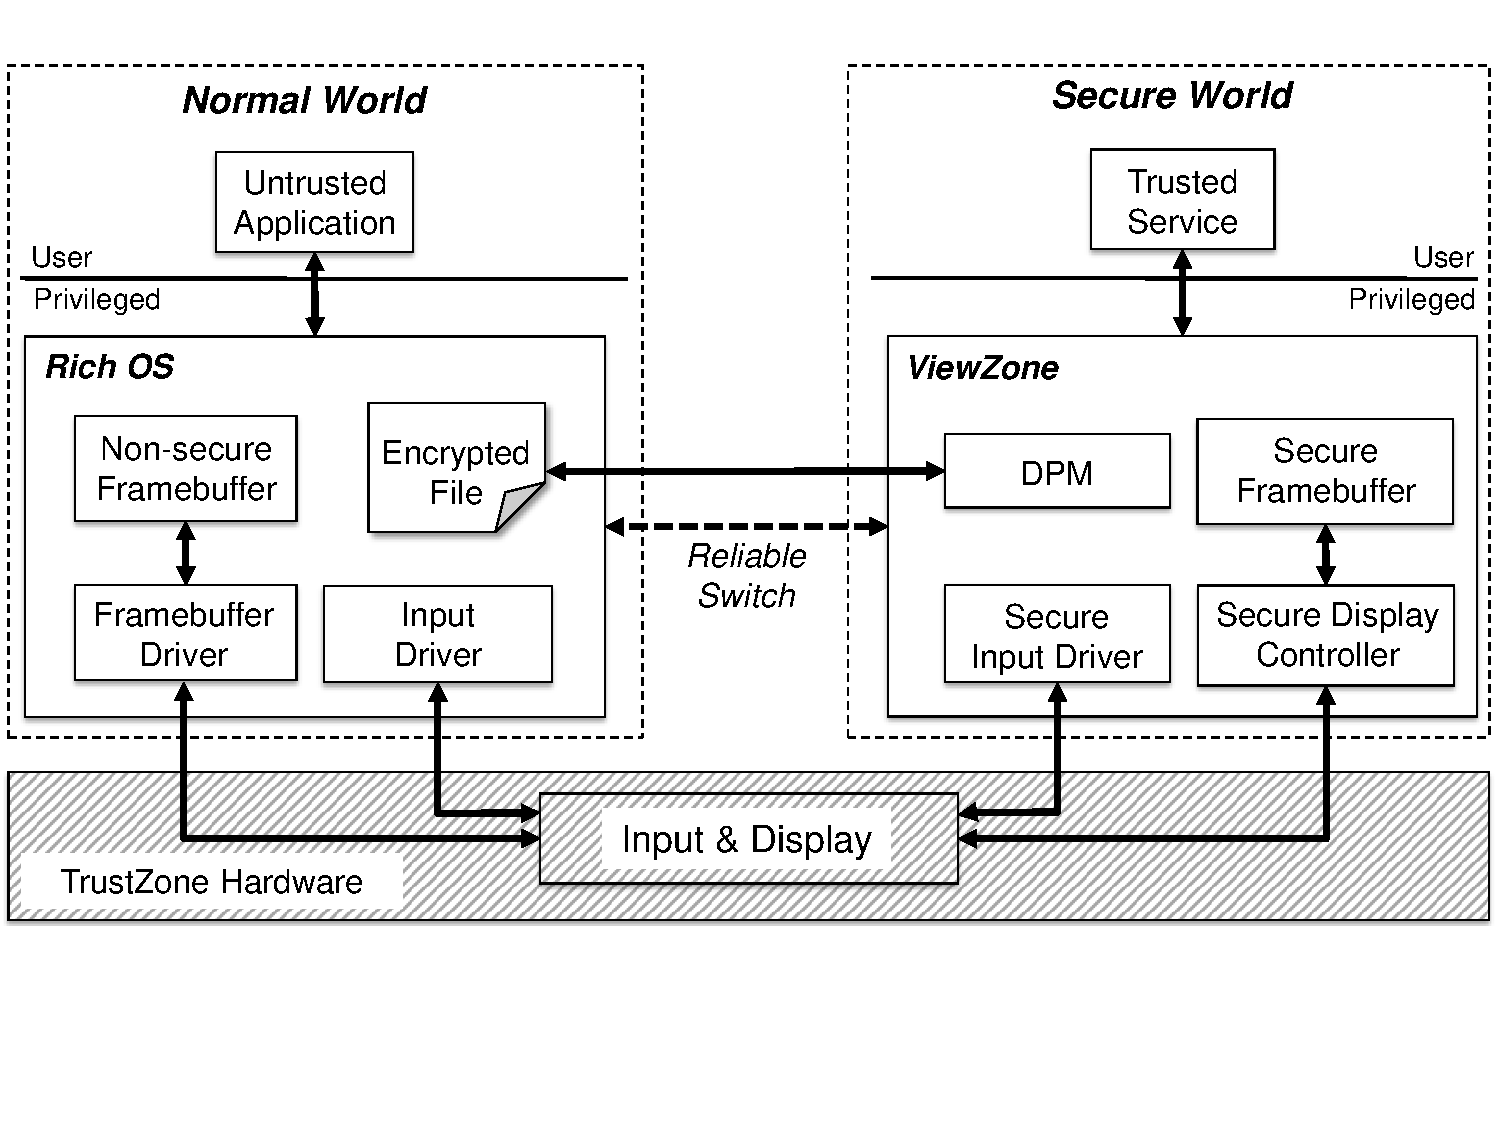
\includegraphics[width=1\textwidth]{img/viewzone_architecture.pdf}
	\caption{ViewZone's Architecture}
	\label{fig:viewzone_architecture}
\end{figure}

\paragraph{\textbf{Architecture}} Figure~\ref{fig:viewzone_architecture} combines all the components, techniques and mechanisms described above into \emph{ViewZone}'s architecture. An untrusted applications running in the rich OS works as a front-end for the trusted service in the secure domain. This untrusted application loads the encrypted sensitive file, whose content is only accessible by the secure world, into a shared memory region. This shared memory region allows the \ac{DPM} to securely copy the encrypted file to an isolated secure memory region so it can be decrypted and later displayed to the user. The \ac{DPM} looks into the shared memory region only when the reliable switch is triggered by the secure \ac{NMI} hardware interrupt, thus assuring the subsequent operations are executed by the secure side, meaning the content displayed is authentic. Once the \ac{DPM} has access to the sensitive file content, the secure display controller copies the non-secure framebuffer to the secure framebuffer and the content of the sensitive file can be integrated with that of the original framebuffer, thus giving the impression of integrated user interface between the untrusted and secure domains. This way, the trusted service can display content as it would be displayed by the original rich OS interface. The input is also controlled by the secure world by using the specific input driver in the trusted domain. When another \ac{NMI} interrupt is triggered, the \ac{DPM} encrypts the file again and returns it to the shared memory region where it was first loaded by the untrusted application, thus allowing the trusted service to edit the file, which will then be stored in the untrusted domain.
%\cleardoublepage
%%!TEX root = ../report.tex

% 
% Evaluation
% 
% (1/2pgs)
\section{Implementation and Evaluation}
\label{sec:evaluation}

This section describes the implementation details of the solution as well as how the system is going to be evaluated. \emph{ViewZone} will run along side Android and will be implemented upon a Freescale i.MX53 Quick Start Board development board\footnote{\url{http://www.freescale.com/products/arm-processors/i.mx-applications-processors-based-on-arm-cores/i.mx53-processors/i.mx53-quick-start-board:IMX53QSB}}, which supports ARM's TrustZone. To fully demonstrate the concept of \emph{ViewZone}, we aim to develop a sensitive mobile health application for displaying Personal Health Records (PHR). This application allows a user to display and store his personal health information securely, without sensitive information ever being exposed to an untrusted rich OS such as Android.

\subsection{Implementation}

\paragraph{The \ac{PHR} application} comprises an untrusted client Android application which loads the sensitive encrypted file to a dedicated memory region shared by both worlds. This file is the personal health record to be displayed to the user. The client application then notifies the user the file is loaded and the user may proceed with the reliable world switch by pressing the button dedicated for the \ac{NMI} interrupt. After this world switch, the file in the shared memory region is decrypted and shown to the user. The file can then be stored securely in the untrusted world by saving it and triggering a new reliable world switch, which encrypts the file and stores it in the untrusted rich OS.

\paragraph{Secure Display} is supported by a self-contained secure display controller in the secure domain and an Image Processing Unit (IPU) driver implemented in the rich OS. When the rich OS is running, the IPU is set as a non-secure device and can transfer data from the non-secure framebuffer to the display device. When the system switches to the secure domain, the secure display controller checks the integrity of the IPU driver, saves its state and resets it as a secure device in order to transfer the data from the secure framebuffer to the display device. Before switching back to the normal world, the controller erases the footprint in the IPU to prevent information leakage, and then restores the device state for the rich OS. This method, which reuses the IPU driver implemented by the rich OS, needs additional code to check the driver's integrity, but maintains a smaller TCB than if a self-contained IPU driver was implemented in the secure world.

\paragraph{Memory Isolation} is possible through a watermarking mechanism available in the i.MX53 QSB. This mechanisms allows the isolation of secure memory regions from non-secure memory ones designated for the rich OS. This memory isolation is necessary for the implementation of the secure framebuffer and to isolate the decrypted file from the normal world domain after the reliable world switch. The i.MX53 QSB has two banks of RAM, each with 512 MB and the watermarking mechanism can watermark one continuous region of up to 256 MB on each bank, totalling 512 MB of possible secure RAM. This is more than enough to support the framebuffer and most regular sized files.

\paragraph{Reliable Switch} is based on the non-maskable interrupt mechanism, but the i.MX53 QSB does not provide any \ac{NMI} explicitly. For this reason an \ac{NMI} needs to be constructed in order to support reliable world switches. To achieve this the interrupt type of the \ac{NMI} must be assigned as secure in the Interrupt Security Register (TZIC\_INTSEC), which prevents the rich OS to modify the configuration of the \ac{NMI}. Then, several configuration bits are set to zero so that the rich OS cannot disable, block or intercept the interrupt request made to the ARM processor. Finally the interrupt source, such as a physical button, must be configured as a secure peripheral.

\subsection{Evaluation}

To evaluate \emph{ViewZone} we will measure the performance overhead for displaying files, as well as compare the development process for the PHR mHealth app using ViewZone and a similar app built on top of Android. The performance can be measured by using the performance monitor available in the Cortex-A8 processor to count the CPU cycles and then convert the cycles to time by multiplying 1 \emph{ns / cycle}. By conducting each experiment for each of the use cases described several times and averaging the value we can compare this value taken for \emph{ViewZone} with the value measured in the same conditions for a similar application without using the secure system. We will also assess the complexity of \emph{ViewZone}'s TCB and the final attack surface.

\section{Future Work Plan}
\label{sec:workplan}

Future work is scheduled as follows:

\begin{itemize}
	\item[$\bullet$] January 9 - March 25: Fully design and implement the proposed architecture, including preliminary tests;
	\item[$\bullet$] March 26 - May 1: Perform the complete experimental evaluation 	of the system;
	\item[$\bullet$] March 26 - May 10: Write a paper describing the project;
	\item[$\bullet$] May 11 - June 15: Write the dissertation;
	\item[$\bullet$] June 15: Deliver the MSc dissertation.
\end{itemize}
%\cleardoublepage
%%!TEX root = ../report.tex

% 
% Conclusions
% 

\section{Conclusions}
\label{sec:conclusion}

Wrap up what you wrote.
%\cleardoublepage

%[PREVIOUS/ORIGINAL CONFIG]
%\newpage
%\appendix
%%!TEX root = ../report.tex

\section{Appendix} % (fold)
\label{sec:attachments}

Appendix files and refs will go here.
Such as your thesis work scheduling. 

\subsection{Work Scheduling Example} % (fold)
\label{sub:work_scheduling}
Simple work schedule is presented in Table~\ref{tab:worktable}. You can do something more fancy link a Gantt chart or whatever.
\begin{table}[H]
  \caption{Work Scheduling}
  \label{tab:worktable}
  \begin{center}
    \begin{tabular}{l|cc}
    \hline

    \hline
    \textbf{Month} & \textbf{Work} \\
    \hline
      February & Do Stuff \\
    \hline
      February & Do Stuff \\
    \hline
      March & Do Stuff   \\
    \hline
      April & Do Stuff   \\
    \hline
      May & Do Stuff   \\
    \hline
      May & Do Stuff   \\
    \hline
      June & Do Stuff   \\
    \hline
      July & Do Stuff   \\
    \hline

    \hline
    \end{tabular}
  \end{center}
\end{table}
%\tableofcontents
%\cleardoublepage


%
% Bibliography
%
\Urlmuskip=0mu plus 1mu
\bibliographystyle{plain}
\addcontentsline{toc}{section}{References}
\bibliography{references}

%\newpage
%\appendix
%%!TEX root = ../report.tex

\section{Appendix} % (fold)
\label{sec:attachments}

Appendix files and refs will go here.
Such as your thesis work scheduling. 

\subsection{Work Scheduling Example} % (fold)
\label{sub:work_scheduling}
Simple work schedule is presented in Table~\ref{tab:worktable}. You can do something more fancy link a Gantt chart or whatever.
\begin{table}[H]
  \caption{Work Scheduling}
  \label{tab:worktable}
  \begin{center}
    \begin{tabular}{l|cc}
    \hline

    \hline
    \textbf{Month} & \textbf{Work} \\
    \hline
      February & Do Stuff \\
    \hline
      February & Do Stuff \\
    \hline
      March & Do Stuff   \\
    \hline
      April & Do Stuff   \\
    \hline
      May & Do Stuff   \\
    \hline
      May & Do Stuff   \\
    \hline
      June & Do Stuff   \\
    \hline
      July & Do Stuff   \\
    \hline

    \hline
    \end{tabular}
  \end{center}
\end{table}
%\tableofcontents

% *** DEFINITION OF ACRONYMS ***
\acrodef{PC}{Personal Computer}
\acrodef{mHealth}{Mobile Health}
\acrodef{OS}{Operating System}
\acrodef{TCB}{Trusted Computing Base}
\acrodef{LOC}{Lines Of Code}
\acrodef{UCLA}{University of California, Los Angeles}
\acrodef{CNN}{Cable News Network}
\acrodef{ARM}{ARM Holdings}
\acrodef{HIPAA}{Health Insurance Portability and Accountability Act}
\acrodef{API}{Application Programming Interface}
\acrodef{DRM}{Digital Rights Management}
\acrodef{DMB}{external-device misbonding}
\acrodef{PHR}{Personal Health Record}
\acrodef{OMA}{Open Mobile Alliance}
\acrodef{DAC}{Discretionary Access Control}
\acrodef{MAC}{Mandatory Access Control}

\end{document}
